%
% section 7.2
%
\setcounter{section}{1}
\section{Περιοχές / Τομείς Διαχείρισης Δικτύου στο Μοντέλο OSI}

Σε δίκτυα μεσαίου και μεγάλου μεγέθους είναι σχεδόν πάντοτε απαραίτητος ο σχεδιασμός και η εγκατάσταση ενός \emph{Συστήματος Διαχείρισης Δικτύου, NMS (Network Management System)}. Ένα τέτοιο σύστημα αποτελείται από υλικό και λογισμικό που επιτρέπει στο διαχειριστή να επιβλέπει (και σε αρκετές περιπτώσεις να ρυθμίζει) τα στοιχεία που αποτελούν το δίκτυο και να ελέγχει για σημεία με προβληματική λειτουργία. Η διαχείριση γίνεται από κεντρικό σημείο, τυπικά από ένα υπολογιστή που έχει οριστεί ως υπολογιστής διαχείρισης (Manager Server).

\begin{figure}[!ht]
 \centering
 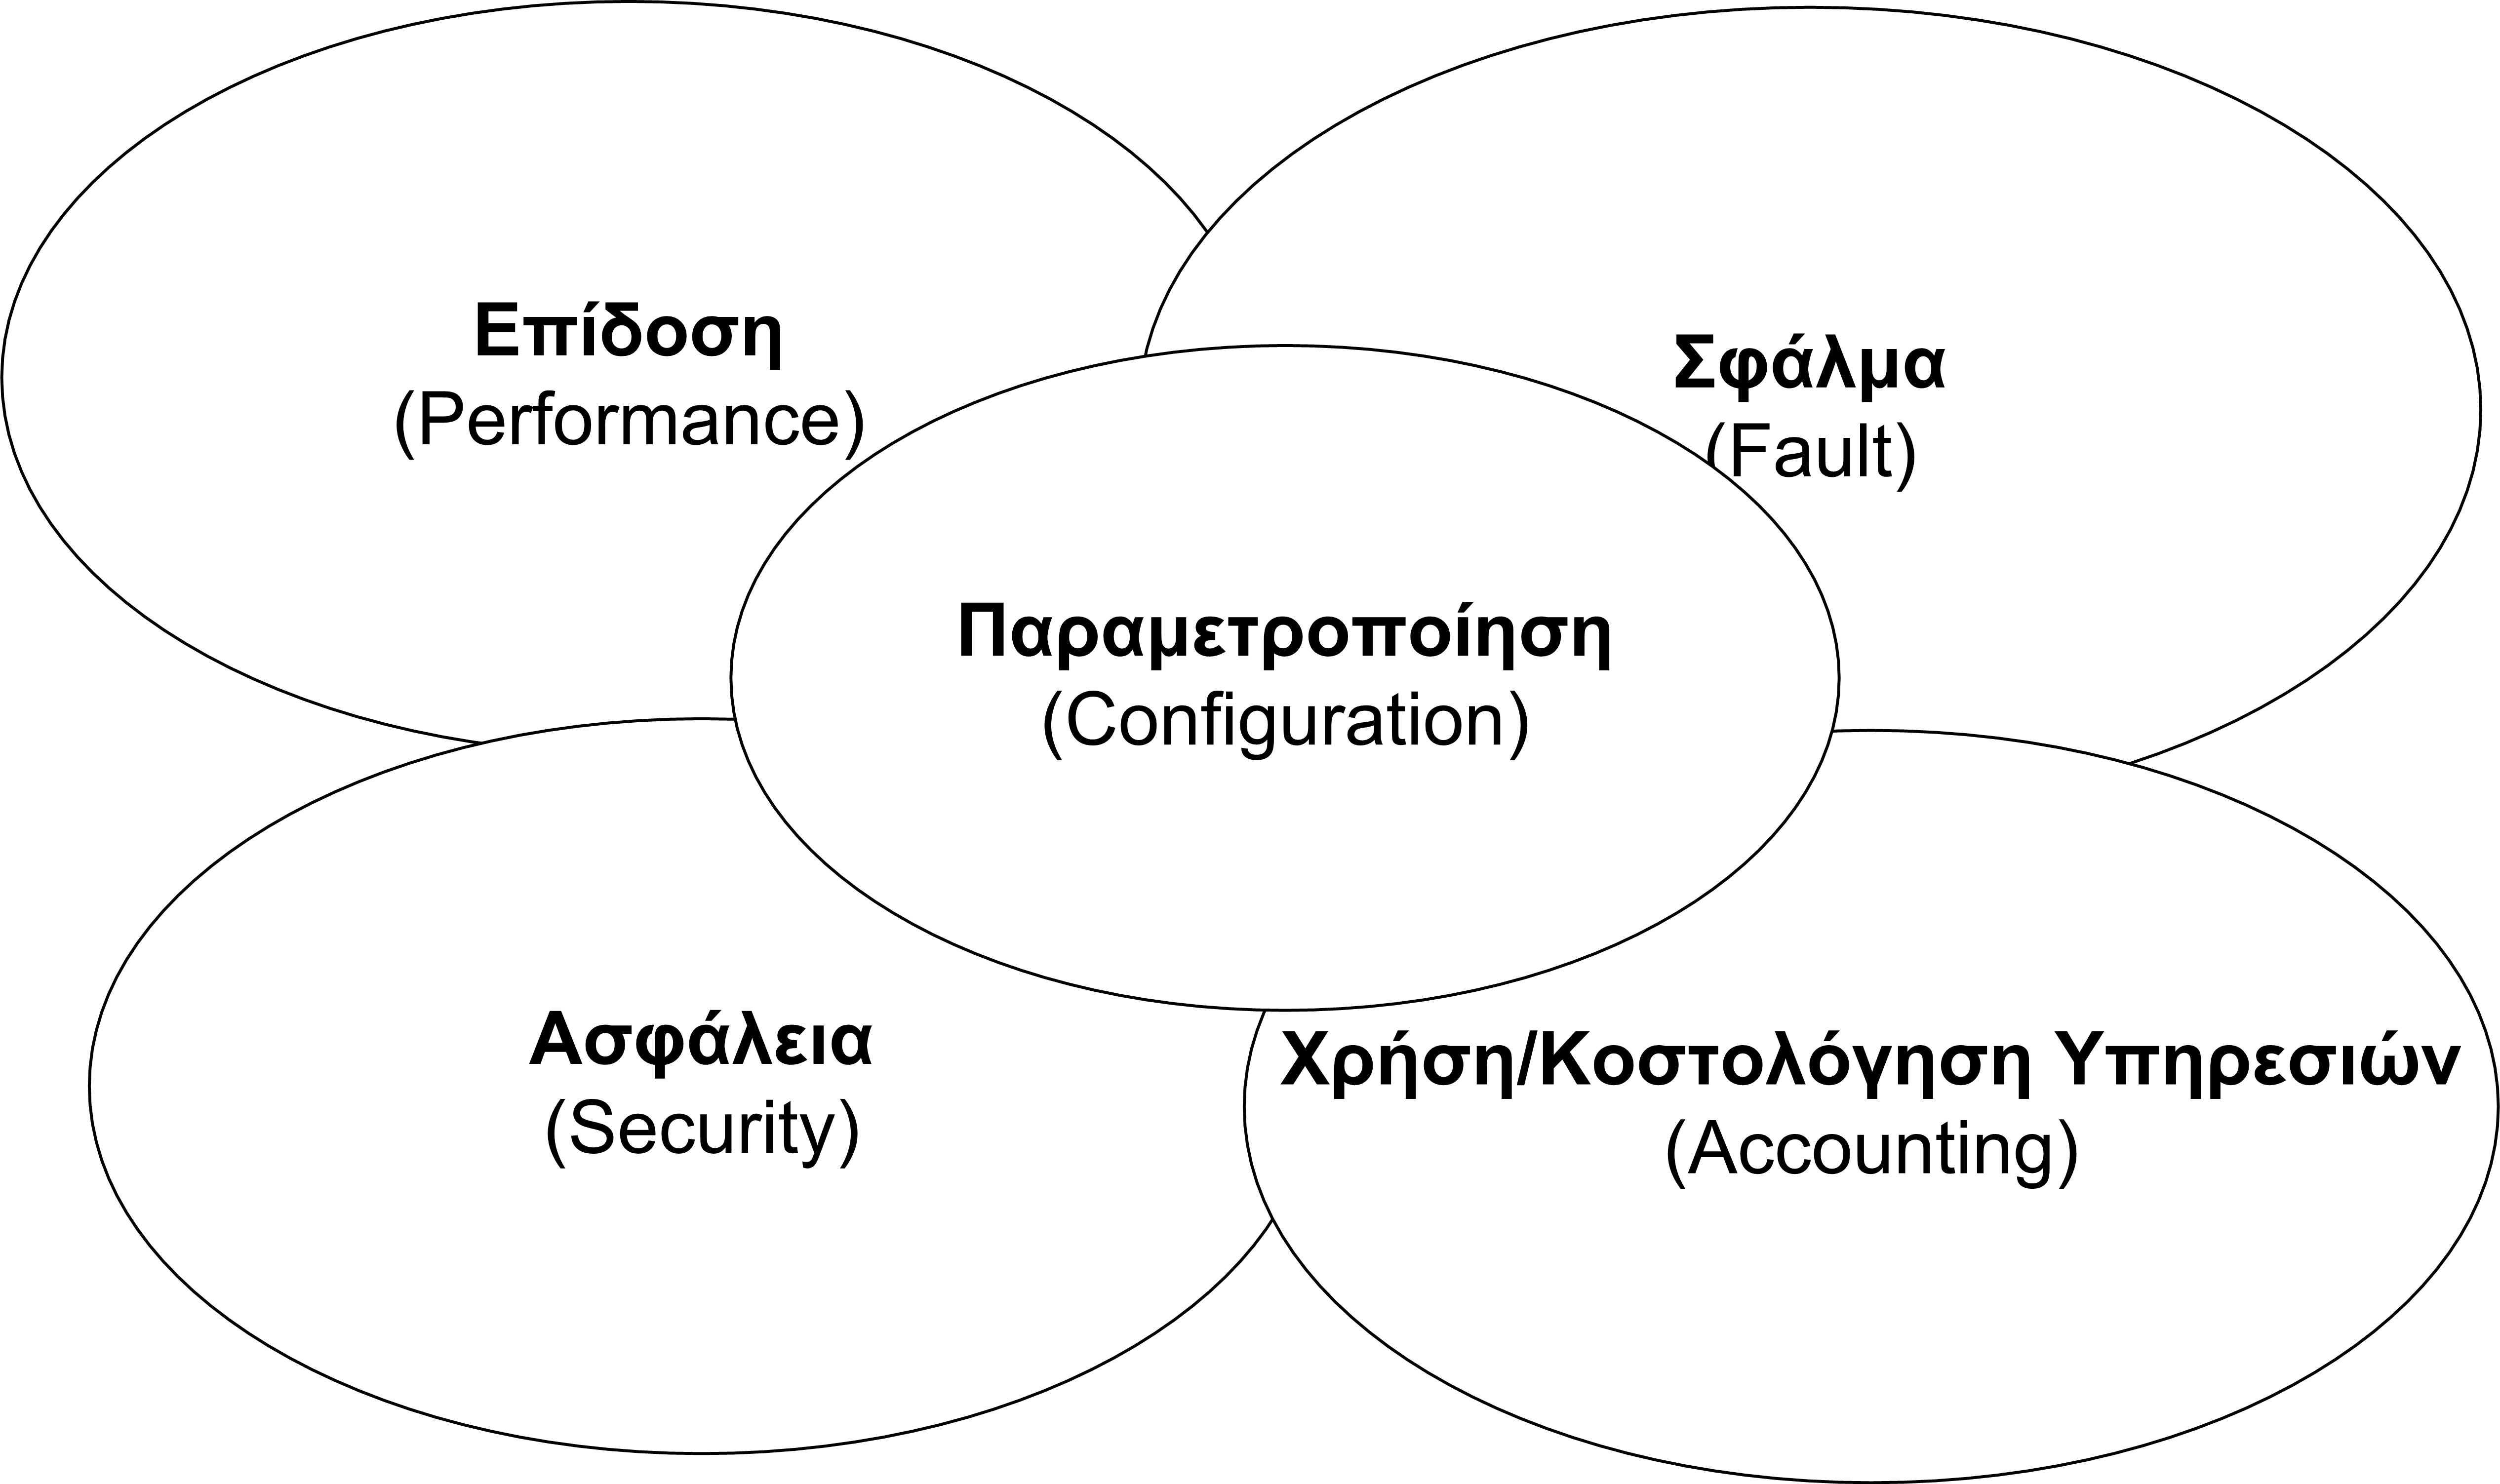
\includegraphics[width=0.95\textwidth]{images/chapter7/7-1}
 \caption {\textsl{Περιοχές Διαχείρισης του OSI}}
 \label{7-1}
\end{figure}

Η Διαχείριση Δικτύου στο μοντέλο OSI χωρίζεται σε πέντε περιοχές, όπως φαίνεται στο σχήμα \ref{7-1}.  Οι περιοχές αυτές είναι:

\begin{itemize}
\item Παραμετροποίηση (Configuration Management)
\item Διαχείριση Σφαλμάτων (Fault Management)
\item Διαχείριση Επιδόσεων (Performance Management)
\item Διαχείριση Κόστους (Accounting Management)
\item Διαχείριση Ασφάλειας (Security Management)
\end{itemize}

Το μοντέλο αυτό ονομάζεται και \emph{FCAPS} από τα αρχικά των λέξεων \emph{Fault Con\-fig\-u\-ra\-tion Accounting Performance Security}. Παρακάτω θα εξηγήσουμε τις διαδικασίες αυτές.